\documentclass[tikz]{standalone}

\usepackage{pgfplots}

\usepackage[utf8]{inputenc}
\usepackage[T1]{fontenc}
\usepackage{times}

\begin{document}

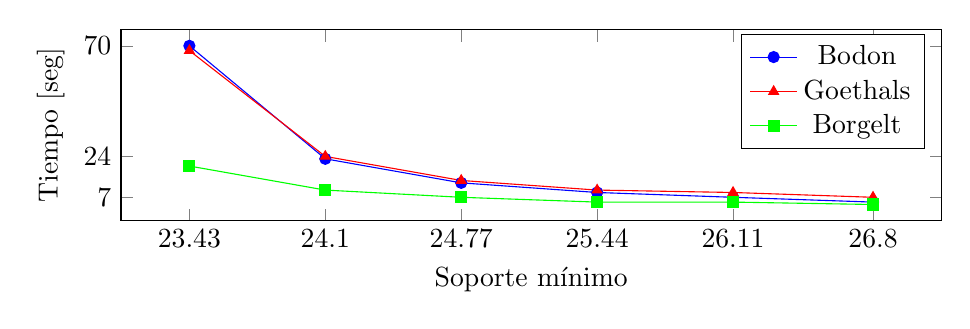
\begin{tikzpicture}
	\begin{axis}[width=12cm,
							height=4cm,
							xtick={26.80,26.11,25.44,24.77,24.10,23.43},
							ytick={7,24,70},
							%title={BMS-View1},
							xlabel={Soporte m\'inimo},
							ylabel={Tiempo [seg]},
							xticklabel style={/pgf/number format/.cd,fixed,precision=3}
							]
		\addplot[color=blue,mark=*] coordinates {(26.8,5) (26.11,7) (25.44,9) (24.77,13) (24.1,23) (23.43,70)};
		\addlegendentry{Bodon}
		\addplot[color=red,mark=triangle*] coordinates {(26.8,7) (26.11,9) (25.44,10) (24.77,14) (24.1,24) (23.43,68)};
		\addlegendentry{Goethals}
		\addplot[color=green,mark=square*] coordinates {(26.8,4) (26.11,5) (25.44,5) (24.77,7) (24.1,10) (23.43,20)};
		\addlegendentry{Borgelt}
	\end{axis}
\end{tikzpicture}

\end{document}
